\section{User-Interface}

Für die Umsetzung des UI wurde das \enquote{Bootstrap} CSS-Framework verwendet. Ausserdem wurden alle
HTML-Templates in der Ruby SLIM templating-language geschrieben, 
welche eine stark vereinfachte Syntax ohne \enquote{Brackets} und ohne \enquote{Closing-Tags} bietet.

\begin{figure}[H]
\begin{codebox}
\begin{minted}{ruby}
.white-box
  .mb-3
    h2.fs-4.mb-1 = t('assessments.new.title')
    span = t('assessments.new.subtitle')
  = render 'assessments/form', assessment: @assessment
\end{minted}
\end{codebox}
\caption{\label{fig:slim-example}Beispiel der SLIM Syntax von }
\end{figure}

Durch diese zwei Mittel und mit der Hilfe der in der Planungsphase erstellten Mockups \ref{}, konnte das UI
rasch umgesetzt werden und ist durch eine klare farbliche Hierarchie ergonomisch strukturiert. Wo nötig, wurden auch
Icons eingesetzt. 

\subsection{Assessments erstellen und verwalten}

\begin{figure}[H]
  \centering
  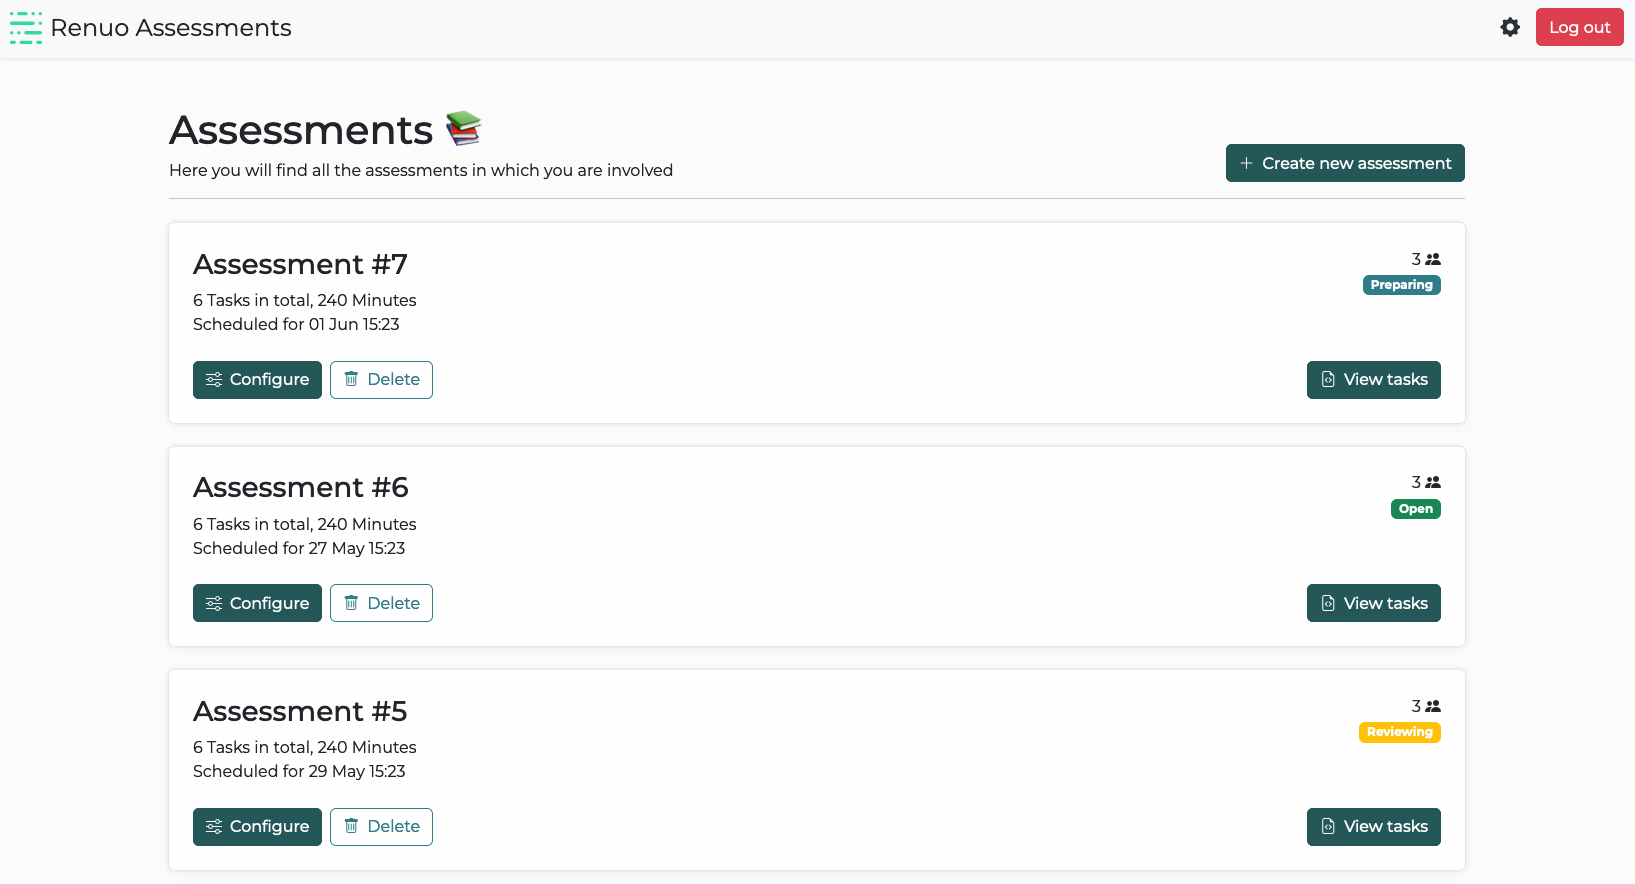
\includegraphics[width=14cm]{images/ui/assessments-index.png}
  \caption{\label{fig:assessments-index}Index-Seite, die alle Assessments auflistet}
\end{figure}

\begin{figure}[H]
  \centering
  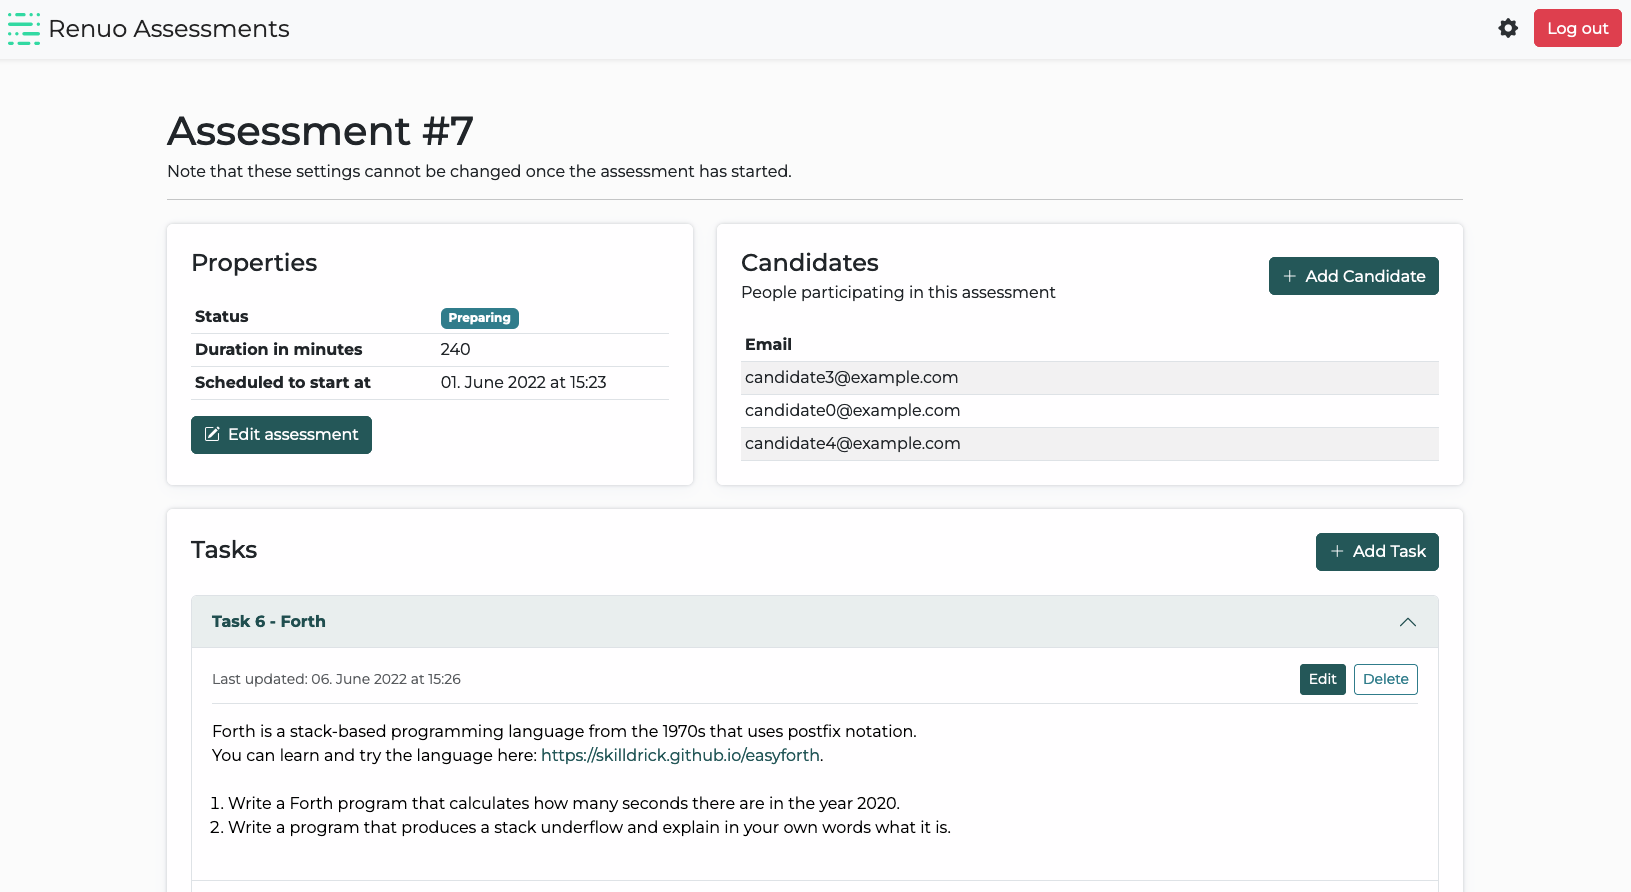
\includegraphics[width=14cm]{images/ui/assessments-edit.png}
  \caption{\label{fig:assessments-edit}}
\end{figure}

\subsection{Assessments lösen}

\subsection{Assessments korrigieren}
